\setlength{\columnsep}{3pt}
\begin{flushleft}
	
	\begin{itemize}
		
		\item \textbf{find}: Searches the directory tree containing a specific file.
		\bigskip
		\begin{tcolorbox}[breakable,notitle,boxrule=-0pt,colback=pink,colframe=pink]
			\color{black}
			\fontdimen2\font=1em
			Syntax: find directory\_name options expression
			\fontdimen2\font=4pt
		\end{tcolorbox}
		Options with \textbf{find} command:
		\bigskip
		\begin{itemize}
			\item \textbf{-name}: Supply an expression to search the directory for.
			\bigskip
			\begin{tcolorbox}[breakable,notitle,boxrule=-0pt,colback=pink,colframe=pink]
				\color{black}
				\fontdimen2\font=1em
				Syntax: find directory\_name -name expression
				\fontdimen2\font=4pt
			\end{tcolorbox}
			Eg: Search for files having name "sample\_file" in directory \textbf{/root}:
			\bigskip
			\begin{tcolorbox}[breakable,notitle,boxrule=-0pt,colback=black,colframe=black]
				\color{green}
				\fontdimen2\font=1em
				\# find /root -name "sample\_file"
				\fontdimen2\font=4pt
			\end{tcolorbox}		
			Special characters in \textbf{-name} option:
			\begin{itemize}
				\item \textbf{"?" in expression}: The question-mark is a wild card which represents 'any one character'.
				\bigskip
				\begin{tcolorbox}[breakable,notitle,boxrule=-0pt,colback=black,colframe=black]
					\color{green}
					\fontdimen2\font=1em
					\# find /root -name "sample?"
					\fontdimen2\font=4pt
				\end{tcolorbox}		
				\item \textbf{"*" in expression}: Represent any number of multiple characters.
				\bigskip
				\begin{tcolorbox}[breakable,notitle,boxrule=-0pt,colback=black,colframe=black]
					\color{green}
					\fontdimen2\font=1em
					\# find /root -name "sample*"
					\fontdimen2\font=4pt
				\end{tcolorbox}		
			\end{itemize}
			
			
			\item \textbf{-user}: Find files owned by a specific user.
			\bigskip
			\begin{tcolorbox}[breakable,notitle,boxrule=-0pt,colback=pink,colframe=pink]
				\color{black}
				\fontdimen2\font=1em
				Syntax: find directory\_name -user user\_name
				\fontdimen2\font=4pt
			\end{tcolorbox}
			\bigskip
			Eg: Find all files/directories owned by user \textbf{"root" in /var directory}.
			\bigskip
			\begin{tcolorbox}[breakable,notitle,boxrule=-0pt,colback=black,colframe=black]
				\color{green}
				\fontdimen2\font=1em
				\# find /var -user root
				\fontdimen2\font=4pt
			\end{tcolorbox}		
			
			\item \textbf{-type}: Find files of specific type like \textbf{file, directory, symbolic link} etc.
			\bigskip
			\begin{tcolorbox}[breakable,notitle,boxrule=-0pt,colback=pink,colframe=pink]
				\color{black}
				\fontdimen2\font=1em
				Syntax: find directory\_name -type [f,d,l,s,c,b]
				\fontdimen2\font=4pt
			\end{tcolorbox}
			\bigskip
			Eg: Find all directories under \textbf{/tmp} directory.
			\bigskip
			\begin{tcolorbox}[breakable,notitle,boxrule=-0pt,colback=black,colframe=black]
				\color{green}
				\fontdimen2\font=1em
				\# find /tmp -type d
				\fontdimen2\font=4pt
			\end{tcolorbox}		
			
			\item \textbf{-atime}: Find files according to their access time.
			\bigskip
			\begin{tcolorbox}[breakable,notitle,boxrule=-0pt,colback=pink,colframe=pink]
				\color{black}
				\fontdimen2\font=1em
				Syntax: find directory\_name -atime [argument]
				\fontdimen2\font=4pt
			\end{tcolorbox}
			\bigskip
			Eg:
			\bigskip
			\begin{tcolorbox}[breakable,notitle,boxrule=-0pt,colback=black,colframe=black]
				\color{yellow}
				\fontdimen2\font=1em
				\# Find files whose access time 3 days hours ago.
				\color{green}
				\newline
				\$ find /tmp –atime 3 
				\newline
				\newline				
				\color{yellow}
				\# Find files whose access time 3 days hours ago and prior to that.
				\color{green}
				\newline
				\$ find /tmp –atime +3 
				\newline
				\color{yellow}
				\newline
				\# Find files whose access time between now and upto 3 days ago.
				\color{green}
				\newline
				\$ find /tmp –atime -3 
				\fontdimen2\font=4pt
			\end{tcolorbox}		
			
			\item \textbf{-perm}: Find files according to specific permission.
			\bigskip
			\begin{tcolorbox}[breakable,notitle,boxrule=-0pt,colback=pink,colframe=pink]
				\color{black}
				\fontdimen2\font=1em
				Syntax: find directory\_name -perm argument
				\fontdimen2\font=4pt
			\end{tcolorbox}
			Eg:
			\bigskip
			\begin{tcolorbox}[breakable,notitle,boxrule=-0pt,colback=black,colframe=black]
				\color{white}
				\fontdimen2\font=1em
				\color{yellow}
				\# Find in the current directory the files having exact permissions of 644.
				\color{green}
				\newline
				\$ find . –perm 644
				\newline
				\color{yellow}
				\newline
				\# Find in the current directory the files having \color{yellow} either rw to user OR r to group OR r to \color{yellow} others. Any one permission match will do.
				\color{green}
				\newline
				\$ find . –perm /644 
				\newline
				\color{yellow}
				\newline
				\# Find in the current directory the files having minimum 664 permissions.
				\color{green}
				\newline
				\$ find . –perm -664
				\fontdimen2\font=4pt
			\end{tcolorbox}		
		\end{itemize}
		
		\bigskip
		\bigskip
		\item \textbf{grep}: Stands for "Global Regular Expression Print". Searches the file for lines containing a match to the given expression.
		\newline
			\begin{tcolorbox}[breakable,notitle,boxrule=-0pt,colback=pink,colframe=pink]
				\color{black}
				\fontdimen2\font=1em
				Syntax: grep expression file\_name
				\fontdimen2\font=4pt
			\end{tcolorbox}
		Eg: Search word "shakher" in file \textbf{/etc/passwd}:
			\bigskip
			\begin{tcolorbox}[breakable,notitle,boxrule=-0pt,colback=black,colframe=black]
				\color{green}
				\fontdimen2\font=1em
				\# grep shakher /etc/passwd
				\newline
				\color{white}
				shakher:x:1000:1000::/home/shakher:/bin/bash
				\newline
				shakher\_suman:x:1000:1000::/home/shakher\_suman:/bin/bash
				\fontdimen2\font=4pt
			\end{tcolorbox}
		Options with \textbf{grep} command:
		\begin{itemize}
			\item \textbf{-i}: Force grep to ignore word case.
			\bigskip
			
			\begin{tcolorbox}[breakable,notitle,boxrule=-0pt,colback=black,colframe=black]
				\color{green}
				\fontdimen2\font=1em
				\# grep -i shakher /etc/passwd
				\newline
				\color{white}
				shakher:x:1000:1000::/home/shakher:/bin/bash
				\newline
				shakher\_suman:x:1000:1000::/home/shakher\_suman:/bin/bash
				\fontdimen2\font=4pt
			\end{tcolorbox}
			
			\item \textbf{-r} or \textbf{-R}: Search recursively i.e. search all files under each directory for a string.
			\bigskip
			\begin{tcolorbox}[breakable,notitle,boxrule=-0pt,colback=black,colframe=black]
				\color{green}
				\fontdimen2\font=1em
				\# grep -r "192.168.1.5" /etc/
				\newline
				\color{white}
				/etc/ppp/options:\# ms-wins 192.168.1.50
				\newline
				/etc/ppp/options:\# ms-wins 192.168.1.51
				\fontdimen2\font=4pt
			\end{tcolorbox}
			
			\item \textbf{-w}: Select only those lines containing matches that form whole words.
			\bigskip
			\begin{tcolorbox}[breakable,notitle,boxrule=-0pt,colback=black,colframe=black]
				\color{green}
				\fontdimen2\font=1em
				\# grep -w "shakher" /etc/passwd
				\newline
				\color{white}
				shakher:x:1000:1000::/home/shakher:/bin/bash
				\fontdimen2\font=4pt
			\end{tcolorbox}

			\item \textbf{-c}: Count a particular word in file.
			\bigskip
			\begin{tcolorbox}[breakable,notitle,boxrule=-0pt,colback=black,colframe=black]
				\color{green}
				\fontdimen2\font=1em
				\# grep -c "Error" logfile.txt
				\newline
				\color{white}
				4
				\fontdimen2\font=4pt
			\end{tcolorbox}
			
			\item \textbf{-n}: Display line number of lines matching the word.
			\bigskip
			\begin{tcolorbox}[breakable,notitle,boxrule=-0pt,colback=black,colframe=black]
				\color{green}
				\fontdimen2\font=1em
				\# grep -n "Error" logfile
				\fontdimen2\font=4pt
			\end{tcolorbox}
			Eg:
			\begin{figure}[h!]
				\centering
				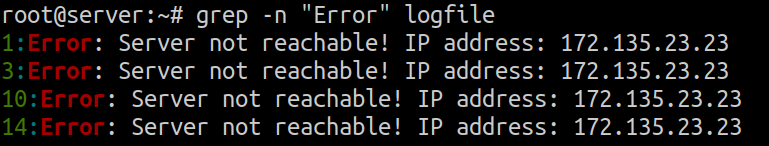
\includegraphics[scale=.4]{content/chapter7/images/grep1.png}
				\caption{Sample output}
				\label{fig:path23}
			\end{figure}

			\item \textbf{-v}: Display only those lines that \textbf{do not} contain the given word.
			\bigskip
			\begin{tcolorbox}[breakable,notitle,boxrule=-0pt,colback=black,colframe=black]
				\color{green}
				\fontdimen2\font=1em
				\# grep -v "nep" logfile
				\fontdimen2\font=4pt
			\end{tcolorbox}		

			\item \textbf{-l}: Displays only the file names which matches the given pattern.
			\begin{tcolorbox}[breakable,notitle,boxrule=-0pt,colback=black,colframe=black]
				\color{green}
				\fontdimen2\font=1em
				\# grep -l "main" *.java
				\fontdimen2\font=4pt
			\end{tcolorbox}					
		\end{itemize}
			Special characters in {grep} command:
			\begin{itemize}
				\item \textbf{\^} : Matches only the lines having the starting word mentioned in the expression.
				\bigskip
				\begin{tcolorbox}[breakable,notitle,boxrule=-0pt,colback=black,colframe=black]
					\color{green}
					\fontdimen2\font=1em
					\# grep -v "\textbf{\^}UUID" /etc/fstab
					\fontdimen2\font=4pt
				\end{tcolorbox}			
				\item \textbf{\$} : Matches only the lines having the last word mentioned in the expression.
				\bigskip
				\begin{tcolorbox}[breakable,notitle,boxrule=-0pt,colback=black,colframe=black]
					\color{green}
					\fontdimen2\font=1em
					\# grep -v "UUID\textbf{\$}" /etc/fstab
					\fontdimen2\font=4pt
				\end{tcolorbox}									
			\end{itemize}
		
		\newpage
				
		\item \textbf{head}: Display starting lines of the file. By default, displays the top 10 lines of file.
		\bigskip
		\begin{tcolorbox}[breakable,notitle,boxrule=-0pt,colback=pink,colframe=pink]
			\color{black}
			\fontdimen2\font=1em
			Syntax: head file\_name
			\fontdimen2\font=4pt
		\end{tcolorbox}
		Eg:
		\bigskip
		\begin{tcolorbox}[breakable,notitle,boxrule=-0pt,colback=black,colframe=black]
			\color{green}
			\fontdimen2\font=1em
			\# head /etc/passwd
			\fontdimen2\font=4pt
		\end{tcolorbox}		
		Options for \textbf{head} command:
		\newline
		\textbf{-n}: Provide the number of lines to be displayed from the start of the file.
		\bigskip
		\begin{tcolorbox}[breakable,notitle,boxrule=-0pt,colback=black,colframe=black]
			\color{green}
			\fontdimen2\font=1em
			\# head -n5 /etc/passwd
			\fontdimen2\font=4pt
		\end{tcolorbox}		

		\bigskip
		\bigskip
		\item \textbf{tail}: Display ending lines of the file. By default, displays the bottom 10 lines of file.
		\bigskip
		\begin{tcolorbox}[breakable,notitle,boxrule=-0pt,colback=pink,colframe=pink]
			\color{black}
			\fontdimen2\font=1em
			Syntax: tail file\_name
			\fontdimen2\font=4pt
		\end{tcolorbox}
		Eg:
		\bigskip
		\begin{tcolorbox}[breakable,notitle,boxrule=-0pt,colback=black,colframe=black]
			\color{green}
			\fontdimen2\font=1em
			\# tail /etc/passwd
			\fontdimen2\font=4pt
		\end{tcolorbox}		
		Options for \textbf{head} command:
		\newline
		\textbf{-n}: Provide the number of lines to be displayed from the end of the file.
		\bigskip
		\begin{tcolorbox}[breakable,notitle,boxrule=-0pt,colback=black,colframe=black]
			\color{green}
			\fontdimen2\font=1em
			\# tail -n5 /etc/passwd
			\fontdimen2\font=4pt
		\end{tcolorbox}		

		\bigskip
		\bigskip
		\item \textbf{more}: Easily read a file without using an editor. \textbf{Press "q"} to quit reading the file.
		\bigskip
		\begin{tcolorbox}[breakable,notitle,boxrule=-0pt,colback=pink,colframe=pink]
			\color{black}
			\fontdimen2\font=1em
			Syntax: more file\_name
			\fontdimen2\font=4pt
		\end{tcolorbox}
		Eg:
		\bigskip
		\begin{tcolorbox}[breakable,notitle,boxrule=-0pt,colback=black,colframe=black]
			\color{green}
			\fontdimen2\font=1em
			\# more /etc/passwd
			\fontdimen2\font=4pt
		\end{tcolorbox}		


		\bigskip
		\bigskip
		\item \textbf{wc}: Display number of \textbf{lines, words and bytes} respectively in a file.
		\bigskip
		\begin{tcolorbox}[breakable,notitle,boxrule=-0pt,colback=pink,colframe=pink]
			\color{black}
			\fontdimen2\font=1em
			Syntax: wc filename
			\fontdimen2\font=4pt
		\end{tcolorbox}
		Eg:
		\bigskip
		\begin{tcolorbox}[breakable,notitle,boxrule=-0pt,colback=black,colframe=black]
			\color{green}
			\fontdimen2\font=1em
			\$ wc myfile
			\newline
			\color{white}
			6 7 39 myfile
			\fontdimen2\font=4pt
		\end{tcolorbox}	

		Options with \textbf{wc} command:
		\begin{itemize}
			\item \textbf{-l}: Display number of lines in a file
			\item \textbf{-w}: Display number of words in a file
			\item \textbf{-c}: Display number of characters in a file
			\newline
			Eg:
			\begin{tcolorbox}[breakable,notitle,boxrule=-0pt,colback=black,colframe=black]
				\color{green}
				\fontdimen2\font=1em
				\# wc -l myfile
				\newline
				\# wc -w myfile
				\newline
				\# wc -c myfile
				\fontdimen2\font=4pt
			\end{tcolorbox}	
		\end{itemize}

		\bigskip
		\bigskip
		\item \textbf{sort}: Sorts file content by default in ascending order.
		\bigskip
		\begin{tcolorbox}[breakable,notitle,boxrule=-0pt,colback=pink,colframe=pink]
			\color{black}
			\fontdimen2\font=1em
			Syntax: sort file\_name
			\fontdimen2\font=4pt
		\end{tcolorbox}
		Eg: Notice the file content \textbf{"phonebook"}:
		\bigskip
		\begin{tcolorbox}[breakable,notitle,boxrule=-0pt,colback=black,colframe=black]
			\color{green}
			\fontdimen2\font=1em
			\$ cat phonebook
			\color{white}
			\newline
			Smith,Brett 5554321
			\newline
			Doe,John 5551234
			\newline
			Doe,Jane 5553214
			\newline
			Avery,Cory 5554321
			\newline
			Fogarty,Suzie 5552314
			\fontdimen2\font=4pt
		\end{tcolorbox}		
		Let's sort the content of \textbf{"phonebook"} file.
		\bigskip
		\begin{tcolorbox}[breakable,notitle,boxrule=-0pt,colback=black,colframe=black]
			\color{green}
			\fontdimen2\font=1em
			\$ sort phonebook
			\color{white}
			\newline
			Avery,Cory 5554321
			\newline
			\color{white}
			Doe,Jane 5553214
			\newline
			\color{white}
			Doe,John 5551234
			\newline
			Fogarty,Suzie 5552314
			\newline
			Smith,Brett 5554321
			\fontdimen2\font=4pt
		\end{tcolorbox}		
		Options with \textbf{sort} command:
		\begin{itemize}
			\item \textbf{-r}: Sort file in reverse order.
			\bigskip
			\begin{tcolorbox}[breakable,notitle,boxrule=-0pt,colback=black,colframe=black]
				\color{green}
				\fontdimen2\font=1em
				\$ sort -r phonebook
				\fontdimen2\font=4pt
			\end{tcolorbox}		
			%\item \textbf{-n}: Makes the program to sort according to numerical value.
		\end{itemize}

		\bigskip
		\bigskip
		\item \textbf{uniq}: Display file content by removing consecutive duplicate lines from the file.
		\bigskip
		\begin{tcolorbox}[breakable,notitle,boxrule=-0pt,colback=pink,colframe=pink]
			\color{black}
			\fontdimen2\font=1em
			Syntax: uniq file\_name
			\fontdimen2\font=4pt
		\end{tcolorbox}
		Eg: Find all unique lines in below file:
		\bigskip
		\begin{tcolorbox}[breakable,notitle,boxrule=-0pt,colback=black,colframe=black]
			\color{green}
			\fontdimen2\font=1em
			\# cat cities.txt
			\newline
			\color{white}
			Pune
			\newline
			Kolhapur
			\newline
			Kolhapur
			\newline
			Pune
			\fontdimen2\font=4pt
		\end{tcolorbox}		
		The \textbf{uniq} command is used find uniq consecutive lines:
		\begin{tcolorbox}[breakable,notitle,boxrule=-0pt,colback=black,colframe=black]
			\color{green}
			\fontdimen2\font=1em
			\# uniq cities.txt
			\newline
			\color{white}
			Pune
			\newline
			Kolhapur
			\newline
			Pune
			\fontdimen2\font=4pt
		\end{tcolorbox}		
		\bigskip
		\bigskip
		\item \textbf{cut}: Extract a certain range of characters from a line or file.
		\newline
		Options with \textbf{cut} command:
		\begin{itemize}
		\item  \textbf{-c}: Display specific character or range of characters.
		\bigskip
		\begin{tcolorbox}[breakable,notitle,boxrule=-0pt,colback=pink,colframe=pink]
			\color{black}
			\fontdimen2\font=1em
			Syntax: cut -cn  file\_name
			\fontdimen2\font=4pt
		\end{tcolorbox}
		Eg: Consider below file:
		\bigskip
		\begin{tcolorbox}[breakable,notitle,boxrule=-0pt,colback=black,colframe=black]
			\color{green}
			\fontdimen2\font=1em
			\# cat company.data
			\newline
			\color{white}
			406378:Sales:Itorre:Jan
			\newline
			031762:Marketing:Nasium:Jim
			\newline
			636496:Research:Ancholie:Mel
			\newline
			396082:Sales:Jucacion:Ed
			\fontdimen2\font=4pt
		\end{tcolorbox}		
		\bigskip
		To display the 6th characters of the file:
		\bigskip
		\begin{tcolorbox}[breakable,notitle,boxrule=-0pt,colback=black,colframe=black]
			\color{green}
			\fontdimen2\font=1em
			\# cut -c6 company.data
			\newline
			\color{white}
			8
			\newline
			2
			\newline
			6
			\newline
			2
			\fontdimen2\font=4pt
		\end{tcolorbox}		
		\bigskip
		Display the range of characters like 2nd to 6th character of the file:
		\bigskip
		\begin{tcolorbox}[breakable,notitle,boxrule=-0pt,colback=black,colframe=black]
			\color{green}
			\fontdimen2\font=1em
			\# cut -c2-6 company.data
			\newline
			\color{white}
			06378
			\newline
			31762
			\newline
			36496
			\newline
			96082
			\fontdimen2\font=4pt
		\end{tcolorbox}		
		\bigskip
		Display only 2nd \& 6th character of the file:
		\bigskip
		\begin{tcolorbox}[breakable,notitle,boxrule=-0pt,colback=black,colframe=black]
			\color{green}
			\fontdimen2\font=1em
			\# cut -c2,6 company.data
			\newline
			\color{white}
			08
			\newline
			32
			\newline
			36
			\newline
			92
			\fontdimen2\font=4pt
		\end{tcolorbox}		
		\item \textbf{-f}: Specifies a field list, the line being cut is supposed to be comprised of fields
		\newline
		\textbf{-d}: The ‘fields’ in the line are determined by delimiter specified by ‘–d ’ option
		\bigskip
		\begin{tcolorbox}[breakable,notitle,boxrule=-0pt,colback=pink,colframe=pink]
			\color{black}
			\fontdimen2\font=1em
			Syntax: cut -fn -d[delimiter]  file\_name
			\fontdimen2\font=4pt
		\end{tcolorbox}
		Eg: \textbf{Cut} 3rd field as per delimiter ":" -
		\bigskip
		\begin{tcolorbox}[breakable,notitle,boxrule=-0pt,colback=black,colframe=black]
			\color{green}
			\fontdimen2\font=1em
			\# cut -d":" -f3 company.data
			\newline
			\color{white}
			Itorre
			\newline
			Nasium
			\newline
			Ancholie
			\newline
			Jucacion
			\fontdimen2\font=4pt
		\end{tcolorbox}		
		Eg: If you want to access multiple fields like 1st and 3rd field, you can separate them by comma:
		\bigskip
		\begin{tcolorbox}[breakable,notitle,boxrule=-0pt,colback=black,colframe=black]
			\color{green}
			\fontdimen2\font=1em
			\# cut -d":" -f1,3 company.data
			\newline
			\color{white}
			406378:Itorre
			\newline
			031762:Nasium
			\newline
			636496:Ancholie
			\newline
			396082:Jucacion
			\fontdimen2\font=4pt
		\end{tcolorbox}				 
	\end{itemize}

		
	\end{itemize}

\end{flushleft}

\newpage

